
\stilian{The purpose of this chapter is to provide a unified review of the fundamental statistical limits in the 
sparse signal detection and support recovery problems.  Our goal is to convey the main ideas and thus we shall focus on 
the simple but important setting of independent Gaussian errors.}{\xout{We study the fundamental limits of the signal detection and support recovery problems in the location models with independent Gaussian errors in this chapter.}}
Specifically, we derive the conditions under which the detection and support recovery problems succeed and fail in the sense of \eqref{eq:support-recovery-success} and \eqref{eq:support-recovery-failure}, in the additive error model 
\begin{equation} \label{eq:model-additive-Chapter3}
    x(i) = \mu(i) + \epsilon(i), \quad i=1,\ldots,p,
\end{equation}
where the errors $\epsilon(i)$'s are \ac{iid} standard Gaussians random variables.
Once again, we restrict our analysis to models with independent and identically distributed Gaussian errors for the 
moment. Both the distributional assumption and the independence assumption will be relaxed substantially in the following chapters.

As laid out in Section \ref{sec:asymptotics}, we work under the asymptotic regime where the problem dimension 
$p$ diverges to infinity.  The set of non-zero entires of the signal vector $\mu = \mu_p$ will be referred
to as its {\em support} and denoted by 
$$
 S_p:=\{i\, :\, \mu(i)\not = 0\}.
$$
We shall assume that the size of the support is
\begin{equation} \label{eq:signal-sparsity-additive}
    |S_p| = \left\lfloor p^{1-\beta} \right\rfloor, \quad \beta\in(0,1],
\end{equation}
where $\beta$ parametrizes the problem sparsity.
The closer $\beta$ is to 1, the sparser the support $S_p$.  
Conversely, when $\beta$ is close to 0, the support is dense with many non-null signals.
We consider one-sided alternatives \eqref{eq:global-test-one-sided}, and parametrize the range of the non-zero (and perhaps unequal) signals with
\begin{equation} \label{eq:signal-size-additive}
    \underline{\Delta} = \sqrt{2\underline{r}\log{p}}
    \le \mu(i) \le
    \overline{\Delta} = \sqrt{2\overline{r}\log{p}}, \quad \text{for all}\;\;i\in S_p,
\end{equation}
for some constants $0<\underline{r}\le\overline{r}\le+\infty$.

% \label{rmk:global-test-boundary}
The parametrization of signal sparsity \eqref{eq:signal-sparsity-additive} and signal sizes \eqref{eq:signal-size-additive} in the Gaussian model was first introduced in \citet{ingster1998minimax}, and later adopted by \cite{hall2010innovated}, \cite{cai2011optimal}, \cite{zhong2013tests}, \cite{cai2014optimal}, \cite{arias2017distribution1}, and numerous others for studying the signal detection problem in Gaussian location-scale models.
Similar scalings of sparsity and signal size are also used in, e.g., \cite{ji2012ups}, \cite{jin2014optimality}, \cite{butucea2018variable} to study the phase transitions of the support recovery problems under Gaussianity assumptions.

\section{Sparse signal detection problems}
\label{sec:global-tests}

The optimality of sparse signal detection was first studied by \citet{ingster1998minimax}, who showed that a phase transition in the $r$-$\beta$ plane exists for the signal detection problem. 
Specifically, assuming equal signal sizes with magnitude $\sqrt{2{r}\log{p}}$, if the signal size $r$ is above a so-called detection boundary,
\begin{equation} \label{eq:detection-boundary-large-signals}
    f(\beta) = 
    \begin{cases}
        \max\{0,\; \beta - 1/2\} & 0 < \beta \le 3/4, \\
        \left(1 - \sqrt{1-\beta}\right)^2 & 3/4 < \beta \le 1,
    \end{cases}
\end{equation} 
then the global null hypothesis $\mu(i)=0$ for all $i=1,\ldots,p$ can be distinguished from the alternative as $p\to\infty$ in the sense of \eqref{eq:support-recovery-success} using the likelihood ratio test; 
otherwise, when signal sizes fall below the boundary, no test can do better than a random guess.
Adaptive tests such as Tukey's \ac{HC} \citep{donoho2004higher} and a modified goodness-of-fit test statistic of \citet{zhang2002powerful} have been identified to attain this performance limit without knowledge of the sparsity and signal sizes. 
% We visualize this boundary $f$ in the upper panel of Figure \ref{fig:phase-diagram-signal-detection}.
It is also known that the max-statistic \eqref{eq:max-statistic} is only efficient when $r>(1+\sqrt{1-\beta})^2$, and is therefore sub-optimal for denser signals where $1/2\le\beta\le 3/4$; see \cite{cai2011optimal}.
In contrast, the sum-of-square-type statistics such as $L_2$ was shown in \cite{fan1996test} to be asymptotically powerless when the $L_2$-norm of the signal $\|\mu\|_2^2$ is $o(\sqrt{p})$, or equivalently, when $\beta>1/2$ in our parametrization.

Notice that the scaling for the signal magnitude $\Delta = \sqrt{2r\log{p}}$ is useful for studying very sparse signals ($\beta>1/2$), but fails to reveal the difficulties of the detection problems when signals are relatively dense ($\beta<1/2$).
Indeed, a different scaling is needed for small but dense signals.
With slight overloading of notation, we parametrize signal sizes as 
\begin{equation} \label{eq:signal-size-small} 
    \underline{\Delta} = p^{\underline{r}}
    \le \mu(i) \le
    \overline{\Delta} = p^{\overline{r}}, \quad \text{for all}\;\;i\in S_p,
\end{equation}
where $\underline{r}$ and $\overline{r}$ are negative constants.
In this scaling for the faint signals, \citet{cai2011optimal} showed that a similar phase transition characterized by the following boundary,
\begin{equation} \label{eq:detection-boundary-small-signals}
    f_s(\beta) = \beta - 1/2, \quad 0 < \beta \le 1/2,
\end{equation} 
exists.
Specifically, if $\overline{r}<f_s(\beta)$, the signal detection fails in the sense of \eqref{eq:support-recovery-failure} regardless of the procedures, while the \ac{HC} statistic continues to attain asymptotically perfect detection when $\underline{r}>f_s(\beta)$. 
We visualize this boundary in the lower panel of Figure \ref{fig:phase-diagram-signal-detection}.

\begin{figure}
      \centering
      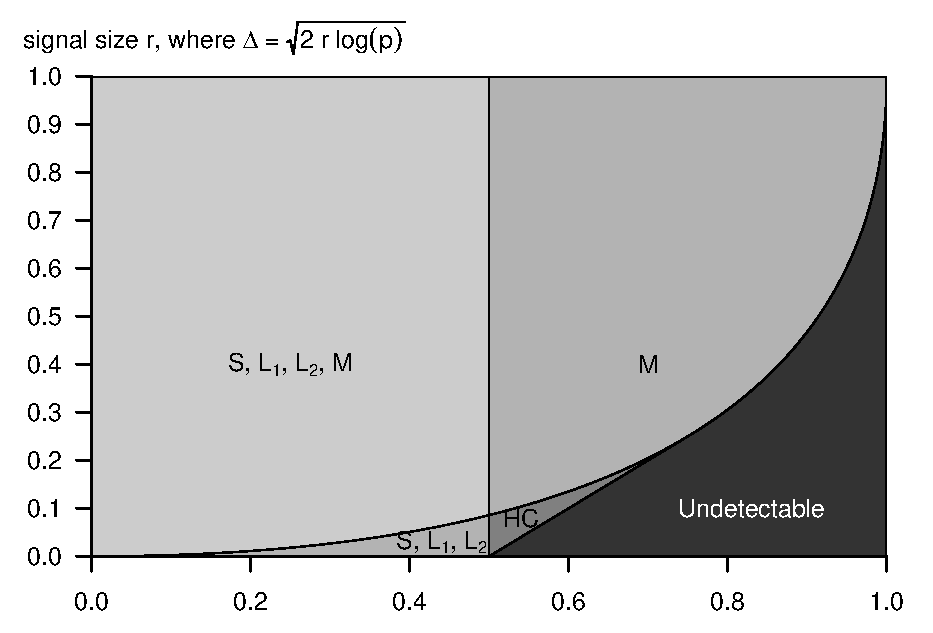
\includegraphics[width=0.7\textwidth]{figures/phase_diagram_signal_detection.eps}
      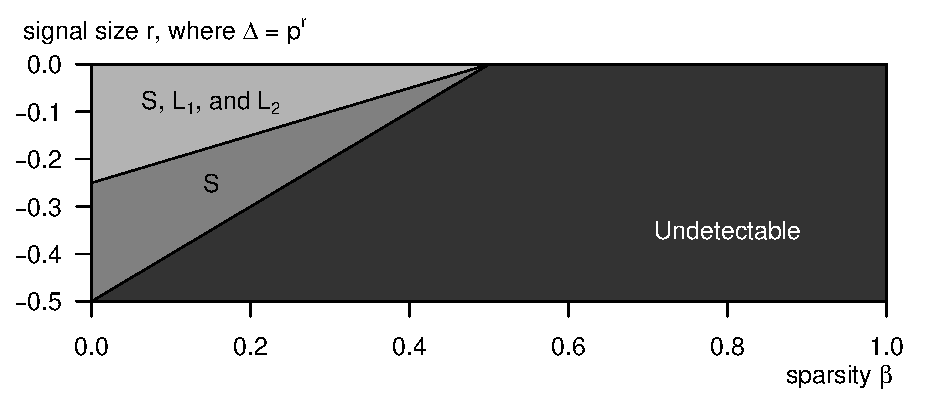
\includegraphics[width=0.7\textwidth]{figures/phase_diagram_signal_detection_vanishing_signals.eps}
      \caption{The phase diagrams of the sparse signal detection problem. 
      Signal size and sparsity are parametrized by $r$ and $\beta$, respectively.
      % Signal sparsity $|S|$ is parametrized by $\beta$. 
      % Signal sizes $\Delta$, parametrized by $r$, increases with dimension $p$ inside the upper panel, and decreases with $p$ inside the power panel.
      The diagrams illustrate the regions where the signal detection problem can be solved asymptotically by some of the commonly used statistics: the maximum ($M$), the sum-of-squares ($L_2$), the sum-of-absolute values ($L_1$), and the sum ($S$).
      In each region of the diagram, the annotated statistics can make the detection risk \eqref{eq:risk-detection} vanish, as dimension $p$ diverges. Conversely, the risks has liminf at least one.
      The detection problem is unsolvable for very sparse and weak signals in the undetectable regions.
      Notice that the $L_1$ and $L_2$ statistics are in fact sub-optimal for all sparsity levels.
      On the other hand, the max-statistic remains powerful for sparse signals ($\beta>1/2$), and is fully efficient when the problem is very sparse ($\beta\ge3/4$).
      The \ac{HC} statistic can detect signals in all configurations in the detectable regions.
      See text and Theorem \ref{thm:detection-optimality}.}
      \label{fig:phase-diagram-signal-detection}
\end{figure}


To the best of our knowledge, performance of simple statistics such as $L_1$, $L_2$ norms, and \stilian{R2, Typo 7.  I suggest writing the following in red, but note that
``S" can be confused with the support.  Can we use $\Sigma$ or ${\rm Sum}$? }{the sum statistic $S$ in \eqref{eq:sum-statistic}}
in this weak signal setting have not been reported in the literature perhaps due to a perceived lack of novelty.
Our first \stilian{Suggest replacing ``Theorem" with ``theorem" and using a capital letter only when we quote a specific Theorem X.Y. -- same for Lemma, Proposition, etc.}{Theorem} investigates the performance of these routine statistics for detecting sparse signals in high-dimensions, and summarizes the known results.

\begin{theorem} \label{thm:detection-optimality}
Consider the signal detection problem in the triangular array of Gaussian error models \eqref{eq:model-additive-Chapter3} where the sparsity is parametrized as in \eqref{eq:signal-sparsity-additive}.
\begin{itemize}
    \item For signals whose sizes are parametrized as in \eqref{eq:signal-size-additive}, the detection problem can be asymptotically solved in the sense of \eqref{eq:support-recovery-success} with $L_2$, $L_1$, or $S$ statistic when $\beta\le 1/2$; on the other hand, these statistics are asymptotically powerless in the sense of \eqref{eq:support-recovery-failure} when $\beta>1/2$.
    \item For small and dense signals whose signal sizes are parametrized as in \eqref{eq:signal-size-small}, the detection problem can be asymptotically solved in the sense of \eqref{eq:support-recovery-success} with $L_2$ or $L_1$ statistic when $\underline{r}>\beta/2-{1}/{4}$; on the other hand, these statistics are asymptotically powerless in the sense of \eqref{eq:support-recovery-failure} when $\overline{r}<\beta/2-{1}/{4}$.
    Further, tests based on the $S$ statistic can succeed asymptotically in the sense of \eqref{eq:support-recovery-success} when $\underline{r}>\beta-1/2$, hence attaining the boundary of detectability in \eqref{eq:detection-boundary-small-signals}.
\end{itemize}
\end{theorem}

Theorem \ref{thm:detection-optimality} is proved in Section \ref{sec:proofs} below.
We visualize the results in Theorem in Figure \ref{fig:phase-diagram-signal-detection}.
It is worth noting that the $\beta$-$r$ parameter regions where $L_1$ and $L_2$ statistics are asymptotically powerful coincide, and these statistics are theoretically suboptimal for both sparse regimes ($\beta>1/2$) and relatively dense regimes ($\beta\le 1/2$).

Ideas have been proposed to combine statistics that are powerful for different alternatives to create adaptive tests that maintain high power for at all sparsity levels.
Such adaptive tests can be constructed, for example, by leveraging the asymptotic independence of the sum- and supremum-type statistics \citep{hsing1995note}. 
Recently, \citet{xu2016adaptive} showed that for dependent observations under mixing and moment conditions, the sum-of-power-type statistics
\begin{equation}
    \widetilde{L}_q(x) = \sum_{i=1}^p x^q(i)
\end{equation} 
with distinct positive integer powers (i.e., $q=1,2,\ldots$) are asymptotically jointly independent, and proposed an adaptive test that monitors the minimium p-value of tests constructed with $\tilde{L}_q$'s.
This idea is further developed in \cite{wu2019adaptive} for generalized linear models and in \cite{he2018asymptotically} with U-statistics.

Optimality properties of such adaptive tests and the optimal choice of the $q$-combinations, however, remain open problems.
\cite{xu2016adaptive} suggested combine $q=1, 2, 3, \ldots, 6$, and  $q=\infty$, based empirical evidence from numerical experiments. 
Theorem \ref{thm:detection-optimality} here implies that, at least for detecting one-sided alternatives, the $\widetilde{L}_2$ statistic (i.e., $L_2$ norm) and the $L_1$ norm are asymptotically dominated by the $\widetilde{L}_1$ statistic (or equivalently, the sum $S$). Therefore it is sufficient to include only the latter in the construction of the adaptive test. 









%\newpage
\section{Sparse signal support recovery problems}
\label{sec:additive-error-model-boundaries}

Turning to support recovery problems in the Gaussian error model \eqref{eq:model-additive-Chapter3},
we will analyze the asymptotic performance limits in terms of the risk metrics for exact, exact-approximate, approximate-exact support recovery problems (i.e., \eqref{eq:risk-exact}, \eqref{eq:risk-exact-approx}, and \eqref{eq:risk-approx-exact}, respectively), as well as the probability of support recovery \eqref{eq:risk-prob}. 
We will also review the recent result for exact support recovery risk \eqref{eq:risk-approximate} by \cite{arias2017distribution}, to reveal a rather complete landscape of support recovery problems in high-dimensional Gaussian error models.

We restrict our attention to the class of thresholding procedures in this section.
Specifically, the lower bounds that we develop in Theorems \ref{thm:Gaussian-error-exact-boundary} through \ref{thm:Gaussian-error-approx-exact-boundary} below are only meant to apply to thresholding procedures. 
Although it is intuitively appealing to consider only data-thresholding procedures in multiple testing problems, such procedures are not always optimal in more general settings. 
% Recently, \cite{arias2019detection} showed that thresholding procedures are in fact sub-optimal in the additive models \eqref{eq:model-additive} when errors have heavy (regularly-varying) tails. 
% Gao and Stoev [14] characterized the conditions under which thresholding procedures are optimal in the exact support recovery problem. 
% The optimality of data-thresholding procedures in terms of other statistical risks is an open problem that invites a dedicated investigation in a future study.
The optimality of thresholding procedures and the consequences of this restriction will be treated in Chapter \ref{chap:exact-support-recovery}.

\medskip

A technical ingredient is needed in order to state our main results.
We define a rate at which the nominal levels of FWER or FDR go to zero.
\begin{definition} \label{def:slowly-vanishing}
We say the nominal level of errors $\alpha = \alpha_p$ vanishes slowly, if
\begin{equation} \label{eq:slowly-vanishing-error}
    \alpha\to 0,\quad \text{and} \quad \alpha p^\delta\to\infty \text{  for any } \delta>0.
\end{equation}
\end{definition}
As an example, the sequence of nominal levels $\alpha_p = 1/\log{(p)}$ is slowly vanishing, while the sequence $\alpha_p = 1/\sqrt{p}$ is not.


\subsection{The exact support recovery problem}
\label{subsec:exact-support-recovery-Gaussian}

Our study of the exact support recovery risk \eqref{eq:risk-exact} begins with a brief review of existing results for the Hamming loss \eqref{eq:Hamming-loss}.
Indeed, as discussions in Section \ref{sec:asymptotics} suggest, the latter can be informative of the exact support recovery problems for models with independent components.

Inspired by the phase transition results for the signal detection problem, \cite{ji2012ups}, \citet{genovese2012comparison}, and \cite{jin2014optimality} derived interesting sharp results on support recovery problems in linear models under the Hamming loss $H(\widehat S, S)$.
Specifically, these papers establish minimax-type phase transition results in their respective settings. 
Under the sparsity parametrization in \eqref{eq:signal-sparsity-additive} and assuming equal signal sizes of ${(2r\log{p})^{1/2}}$, Hamming losses were shown to diverge to $+\infty$ when $r$ falls below the threshold
\begin{equation} \label{eq:strong-classification-boundary-Gaussian}
    g(\beta) = (1 + (1 - \beta)^{1/2})^2,
\end{equation}
for any method of support estimation.
Conversely, under orthogonal, or near-orthogonal random designs, if $r>g(\beta)$, they showed that the methods they proposed achieve vanishing Hamming loss.

Very recently, \citet{butucea2018variable}\; studied both asymptotics and non-asymptotics of support recovery problems in the additive noise model \eqref{eq:model-additive-Chapter3} under the assumption of equal signal sizes, using the Hamming loss.
Again, the analysis of asymptotic optimality focused on a newly proposed procedure which is very specific to the Gaussian model.
It is not at all clear if the optimality properties are a consequence of its mysterious construction.

We now show that commonly used and computationally efficient procedures can also be asymptotically optimal in the exact support recovery problem.

\begin{theorem} \label{thm:Gaussian-error-exact-boundary}
Consider the high-dimensional additive error model \eqref{eq:model-additive-Chapter3} under independent standard Gaussian errors, with signal sparsity and size as described in \eqref{eq:signal-sparsity-additive} and \eqref{eq:signal-size-additive}.
The function \eqref{eq:strong-classification-boundary-Gaussian} characterizes the phase transition of the exact support recovery problem.
Specifically, if $\underline{r} > {{g}}(\beta)$, then Bonferroni's, Sid\'ak's, Holm's, and Hochberg's procedures with slowly vanishing  nominal FWER levels (as defined in Definition \ref{def:slowly-vanishing}) all achieve asymptotically exact support recovery in the sense of \eqref{eq:support-recovery-success}. 

Conversely, if $\overline{r} < {{g}}(\beta)$, then for any thresholding procedure $\widehat{S}_p$, we have $\P[\widehat{S}_p=S_p]\to0$.
Therefore, in view of Lemma \ref{lemma:risk-exact-recovery-probability}, exact support recovery asymptotically fails for all thresholding procedures in the sense of \eqref{eq:support-recovery-failure}.
\end{theorem}

We visualize the result in a $\beta$-$r$ phase diagram in Figure \ref{fig:phase-Gaussian-errors}.

Theorem \ref{thm:Gaussian-error-exact-boundary} is in fact a special case of the more general Theorem \ref{thm:sufficient} which covers dependent and non-Gaussian errors.
We will study the exact support recovery problem in greater detail, and prove the more general version of the Theorem in Chapter \ref{chap:exact-support-recovery}. 

\begin{figure}
  \begin{center}
    \includegraphics[width=0.7\textwidth]{./figures/phase_diagram_Gaussian_ALL_boundaries.eps}
  \end{center}
   \caption{The phase diagram of support recovery problems for the high-dimensional chi-square model \eqref{eq:model-additive-Chapter3}, illustrating the boundaries of the exact support recovery (FWER + FWNR; top curve; Theorem \ref{thm:Gaussian-error-exact-boundary}), the approximate-exact support recovery (FDR + FWNR; second curve from top; Theorem \ref{thm:Gaussian-error-approx-exact-boundary}), the exact-approximate support recovery (FWER + FNR; horizontal line $r=1$; Theorem \ref{thm:Gaussian-error-exact-approx-boundary}), and the approximate support recovery problems (FDR + FNR; tilted line $r=\beta$; Theorem \ref{thm:Gaussian-error-approx-boundary}). The signal detection problem (Type I + Type II errors of the global test; lower curve) was studied in Donoho and Jin (2004). In each region of the diagram and above, the annotated statistical risk can be made to vanish, as dimension $p$ diverges. Conversely, the risks has liminf at least one.}
   \label{fig:phase-Gaussian-errors}
\end{figure}


\subsection{The approximate support recovery problem}
\label{subsec:approx-support-recovery-Gaussian}

\cite{arias2017distribution} studied the performance of the Benjamini-Hochberg procedure \citep{benjamini1995controlling} and a stripped-down version of the Cand\'es-Barber procedure \citep{barber2015controlling} in approximate support recovery problems when the components of the noise term $\epsilon$ in \eqref{eq:model-additive-Chapter3} have independent and symmetric distributions.
A phase transition phenomenon for the approximate support recovery risk \eqref{eq:risk-approximate} was established in the Gaussian additive error model, where the two aforementioned methods are both shown to be asymptotically optimal.

The analysis therein, however, assumed equal signal sizes for the alternatives.
We generalize the main results of \citet{arias2017distribution} to allow for unequal signal sizes.

\begin{theorem} \label{thm:Gaussian-error-approx-boundary}
In the context of Theorem \ref{thm:Gaussian-error-exact-boundary}, the function 
\begin{equation} \label{eq:approx-boundary-Gaussian}
    h(\beta) = \beta
\end{equation}
characterizes the phase transition of approximate support recovery problem.
Specifically, if $\underline{r} > {h}(\beta)$, then the Benjamini-Hochberg procedure (defined in Section \ref{sec:statistical-procedures}) with slowly vanishing nominal FDR levels (as defined in Definition \ref{def:slowly-vanishing}) achieves asymptotically approximate support recovery in the sense of \eqref{eq:support-recovery-success}. 

Conversely, if $\overline{r} < {h}(\beta)$, then approximate support recovery asymptotically fails in the sense of \eqref{eq:support-recovery-failure} for all thresholding procedures.
\end{theorem}

Proof of Theorem \ref{thm:Gaussian-error-approx-boundary} is presented in Section \ref{sec:proofs}. 
The key to proving this generalization is a monotonicity property of the \ac{BH} procedure. 
Namely, the power of the \ac{BH} procedure in terms of FNR monotonically increases for stochastically larger alternatives.
This fact will be formalized in Lemma \ref{lemma:monotonicity-BH-procedure}, and may be of independent interest.

\subsection{The exact-approximate support recovery problem}
\label{subsec:exact-approx-support-recovery-Gaussian}

We now derive two new asymptotic phase transition results for the \emph{asymmetric} statistical risks, \eqref{eq:risk-exact-approx} and \eqref{eq:risk-approx-exact}, in the Gaussian error models.
The next theorem describes the phase transition in the exact-approximate support recovery problem.

\begin{theorem} \label{thm:Gaussian-error-exact-approx-boundary}
In the context of Theorem \ref{thm:Gaussian-error-exact-boundary}, the function 
\begin{equation} \label{eq:exact-approx-boundary-Gaussian}
    \widetilde{g}(\beta) = 1
\end{equation}
characterizes the phase transition of exact-approximate support recovery problem.
Specifically, if $\underline{r} > \widetilde{g}(\beta)$, then the procedures listed in Theorem \ref{thm:Gaussian-error-exact-boundary} with slowly vanishing nominal FWER levels (as defined in Definition \ref{def:slowly-vanishing}) achieve asymptotically exact-approximate support recovery in the sense of \eqref{eq:support-recovery-success}. 

Conversely, if $\overline{r} < \widetilde{g}(\beta)$, then for any thresholding procedure $\widehat{S}$, the exact-approximate support recovery fails in the sense of \eqref{eq:support-recovery-failure}.
\end{theorem}

Theorem \ref{thm:Gaussian-error-exact-approx-boundary} is proved in Section \ref{sec:proofs}. 
The phase transition boundary \eqref{eq:exact-approx-boundary-Gaussian} is visualized in Figure \ref{fig:phase-Gaussian-errors}.


\begin{remark}
Boundary \eqref{eq:exact-approx-boundary-Gaussian} was briefly suggested by \citet{arias2017distribution}.
Unfortunately, it was falsely claimed that the boundary characterized the phase transition of the \emph{exact} support recovery problem, and the alleged proof was left as an ``exercise to the reader''.
This exercise was completed in Chapter \ref{chap:exact-support-recovery}, where the correct boundary \eqref{eq:exact-boundary-chisquared} was identified. 

Theorem \ref{thm:Gaussian-error-exact-approx-boundary} here shows that the boundary \eqref{eq:exact-approx-boundary-Gaussian} \emph{does} exist, though for the slightly different \emph{exact-approximate} support recovery problem.
As we will see in Section \ref{sec:chisq-boundaries}, the boundary \eqref{eq:exact-approx-boundary-Gaussian} also applies to the exact-approximate support recovery problem in chi-square models \eqref{eq:model-chisq}.
\end{remark}

\subsection{The approximate-exact support recovery problem}
\label{subsec:aprox-exact-support-recovery-Gaussian}

The last phase transition is in terms of the approximate-exact support recovery risk
\eqref{eq:risk-approx-exact}.

\begin{theorem} \label{thm:Gaussian-error-approx-exact-boundary}
In the context of Theorem \ref{thm:Gaussian-error-exact-boundary}, the function 
\begin{equation} \label{eq:approx-exact-boundary-Gaussian}
    \widetilde{h}(\beta) = \left(\sqrt{\beta} + \sqrt{1-\beta}\right)^2
\end{equation}
characterizes the phase transition of approximate-exact support recovery problem.
Specifically, if $\underline{r} > \widetilde{h}(\beta)$, then the Benjamini-Hochberg procedure with slowly vanishing nominal FDR levels (as defined in Definition \ref{def:slowly-vanishing}) achieves asymptotically approximate-exact support recovery in the sense of \eqref{eq:support-recovery-success}. 

Conversely, if $\overline{r} < \widetilde{h}(\beta)$, then for any thresholding procedure $\widehat{S}$, the approximate-exact support recovery fails in the sense of \eqref{eq:support-recovery-failure}.
\end{theorem}

Theorem \ref{thm:Gaussian-error-approx-exact-boundary} is proved in Section \ref{sec:proofs}.
The phase transition boundary \eqref{eq:approx-exact-boundary-Gaussian} is visualized in Figure \ref{fig:phase-Gaussian-errors}.


\subsection{Asymptotic power analysis}
\label{subsec:power-analysis}

Theorems \ref{thm:Gaussian-error-exact-boundary} through \ref{thm:Gaussian-error-approx-exact-boundary} allow us to asymptotically quantify the required signals sizes in support recovery problems, as well as in the global hypothesis testing problem in the Gaussian additive error model \eqref{eq:model-additive-Chapter3}. 
Specifically, these results indicate that at all sparsity levels $\beta\in(0,1)$, the difficulties of the problems in terms of the required signal sizes have the following ordering
$$
f(\beta) < h(\beta) < \widetilde{g}(\beta) < \widetilde{h}(\beta) < g(\beta),
$$
as previewed in Figure \ref{fig:phase-Gaussian-errors}.
The ordering aligns with our intuition that the required signal sizes must increase as we move from detection to support recovery problems.
Similarly, more stringent criteria for error control (e.g., FWER compared to FDR) require larger signals.
We can now also compare $\widetilde{g}(\beta)$ and $\widetilde{h}(\beta)$, whose ordering may not be clear from this line of reasoning.


\medskip

Our last comment is on the gap between FDR and FWER under sparsity assumptions. 
Although it is believed that FWER control is sometimes too stringent compared to, say, FDR control in support recovery problems, the fact that all three thresholds (detection, weak, and strong classification) involve the same scaling indicates that the difficulties of the three problems (signal detection, approximate, and exact support recovery) are comparable when signals are very sparse, i.e., when $\beta$ is close to 1.
This is illustrated with the next example.

\begin{example}[Power analysis for variable selection] \label{exmp:gap-when-signal-sparse}
For Gaussian errors (AGG with $\nu = 2$), when $\beta = 3/4$, the signal detection boundary \eqref{eq:detection-boundary-large-signals} says that signals will have to be at least of magnitude $\sqrt{(\log{p})/2}$, 
while approximate support recovery \eqref{eq:approx-boundary-Gaussian} requires signal sizes of at least $\sqrt{3(\log{p})/2}$, 
and exact support recovery \eqref{eq:strong-classification-boundary-Gaussian} calls for signal sizes of at least $\sqrt{9(\log{p})/2}$. 
The required signal sizes increases, but are within the same order of magnitude.

If $m$ independent copies $x_1,\ldots,x_m$ of the observations were made on the same set of $p$ locations, then by taking location-wise averages, $\overline{x}_{m}(j) = \frac{1}{m}\sum_{i=1}^{m} x_i(j)$,
we can reduce error standard deviation, and hence boost the signal-to-noise ratio, by a factor of $\sqrt{m}$.
By the simple calculations above, if $m$ samples are needed to detect (sparse) signals of a certain magnitude, then $3m$ samples will enable approximate support recovery with FDR control, and in fact, $9m$ samples would enable exact support recovery with FWER control.
\end{example}

On the other hand, the gap between FDR and FWER is much larger when signals are dense.
For example, if the signals are only \emph{approximately} sparse, i.e., having a few components above \eqref{eq:strong-classification-boundary-Gaussian} but many smaller components above  \eqref{eq:approx-boundary-Gaussian}, then FDR-controlling procedures will discover substantially larger proportion of signals than FWER-controlling procedures.

Indeed, as $\beta\to0$, the required signal size for approximate support recovery \eqref{eq:approx-boundary-Gaussian} tends to 0, while the required signal size for exact support recovery \eqref{eq:strong-classification-boundary-Gaussian} tends to $4$ in the Gaussian error models.
While Example \ref{exmp:gap-when-signal-sparse} indicates that the exact support recovery is not much more stringent than approximate support recovery when signals are sparse, the gap between required signal sizes widens when signals are dense. 




%\section{Proofs}
%\label{sec:proofs}
%
We first recall some basic properties of the Gaussian distribution in Section \ref{sec:Gaussian-distributions}.
Section \ref{suppsec:BH-monotonicity} states and proves an interesting property of the \ac{BH} procedure which may be of independent interest.
Results on the signal detection problem (Theorem \ref{thm:detection-optimality}) are proved in Section \ref{subsec:proof-additive-error-detection-boundaries}, and the phase transition results on the support recovery problems (Theorems \ref{thm:Gaussian-error-exact-boundary} through \ref{thm:Gaussian-error-approx-exact-boundary}) are shown in Sections \ref{subsec:proof-additive-error-approx-boundaries} and \ref{subsec:proof-additive-error-mix-boundaries}.


\section{Auxiliary facts of Gaussian distributions}
\label{sec:Gaussian-distributions}

We recall three facts of Gaussian distributions that will be used in the proofs later.

We first state the relative stability of iid standard Gaussian random variables,
Since the standard Gaussian distribution falls in the class of asymptotically generalized Gaussians (AGG; see Definition \ref{def:AGG}), by Example \ref{exmp:AGG}, we know that the triangular array ${\cal E} = \{\left(\epsilon_p(i)\right)_{i=1}^p, p\in\N\}$ has relatively stable (RS) maxima in the sense of \eqref{eq:RS-condition}, i.e.,
\begin{equation} \label{eq:relative-stability-Gaussian-maxima}
    \frac{1}{u_{p}} \max_{i=1,\ldots,p} \epsilon_p(i) \xrightarrow{\P} 1,\quad \text{as }\;p\to\infty,
\end{equation}
where $u_p$ is the $(1/p)$-th upper quantile as defined in \eqref{eq:AGG-quantiles}.
Similarly, since the array ${\cal E}$ has distributions symmetric around 0, it also has relatively stable minima
\begin{equation} \label{eq:relative-stability-Gaussian-minima}
    \frac{1}{u_{p}} \min_{i=1,\ldots,p} \epsilon_p(i) \xrightarrow{\P} -1,\quad \text{as }\;p\to\infty.
\end{equation}

The second fact is on the well-known bounds for the Mill's ratio of Gaussian tails.
Let $\Phi$ denote the CDF of the standard Gaussian distribution and $\phi$ its density.
One can show that for all $x>0$ we have
\begin{equation} \label{eq:Mills-ratio}
    \frac{x}{1+x^2}\phi(x) \le \overline{\Phi}(x) = 1-\Phi(x) \le \frac{1}{x}\phi(x),
\end{equation}
using e.g., integration by parts.

The third fact is the stochastic monotonicity of the Gaussian location family. 
In fact, for all location families $\{F_\delta(x)\}_\delta$ where $F_\delta(x) = F(x-\delta)$, we have,
\begin{equation} \label{eq:stochastic-monotonicity-Gaussian}
    F_{\delta_1}(t) \ge F_{\delta_2}(t), \quad \text{for all}\quad t\in\mathbb{R}\quad\text{and all}\quad \delta_1 \le \delta_2.
\end{equation}
Relation \eqref{eq:stochastic-monotonicity-Gaussian} holds, of course, when $F$ is the standard Gaussian distribution. 




\section{Proof of Theorem \ref{thm:detection-optimality}}
\label{subsec:proof-additive-error-detection-boundaries}







\section{Proof of Theorem \ref{thm:Gaussian-error-approx-boundary}}
\label{subsec:proof-additive-error-approx-boundaries}












\section{Proof of Theorems \ref{thm:Gaussian-error-exact-approx-boundary} and \ref{thm:Gaussian-error-approx-exact-boundary}}
\label{subsec:proof-additive-error-mix-boundaries}







